% !TEX root = ../Rulebook.tex
\newpage
\section{Rotating Table Test}
\robin{\st{Conveyor Belt Test / }}

\paragraph{Purpose and Focus of the Test}
The purpose of the \iaterm{Rotating Table Test}{RTT} is to assess the robot's ability to manipulate moving objects which are placed on a \robin{\st{conveyor belt and/or}} rotating turntable. The test demands fast perception and manipulation skills in order to pick up objects from a moving surface.

\paragraph{Scenario Environment}
The same arena as for the Basic Manipulation Test is used. In case that the arena does not already include such a device (see Figure \ref{fig:conveyor_belt}), it will be added only for this particular test.
\robin{\st{The OC may choose to use a rotating turntable instead of a linear conveyor belt in order to simplify the setup of the arena. The particular choice shall be announced before the competition.
An area besides the conveyor belt is left free so that a robot can drive there and grasp the objects from the belt. The other sides might not be accessible, because the device is placed into a corner. 
The conveyor belt should have a wireless mechanism to turn it on.}}

\begin{figure} [h!]
	\begin{center}
%		\subfloat[Conveyor belt]{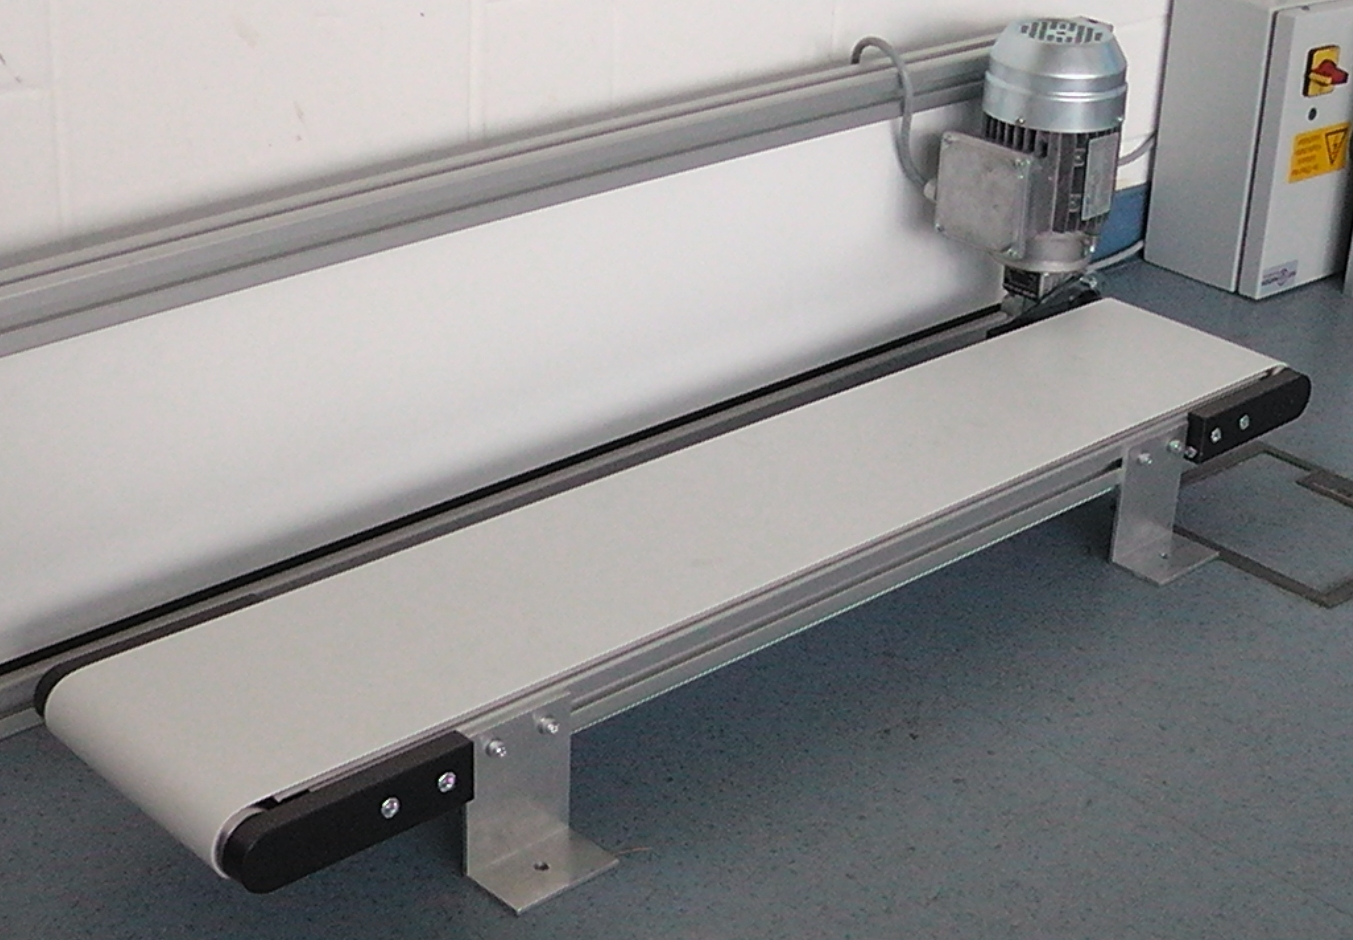
\includegraphics[height = 4cm]{./images/conveyor_belt.jpg}} 
%		\hspace{1cm}
		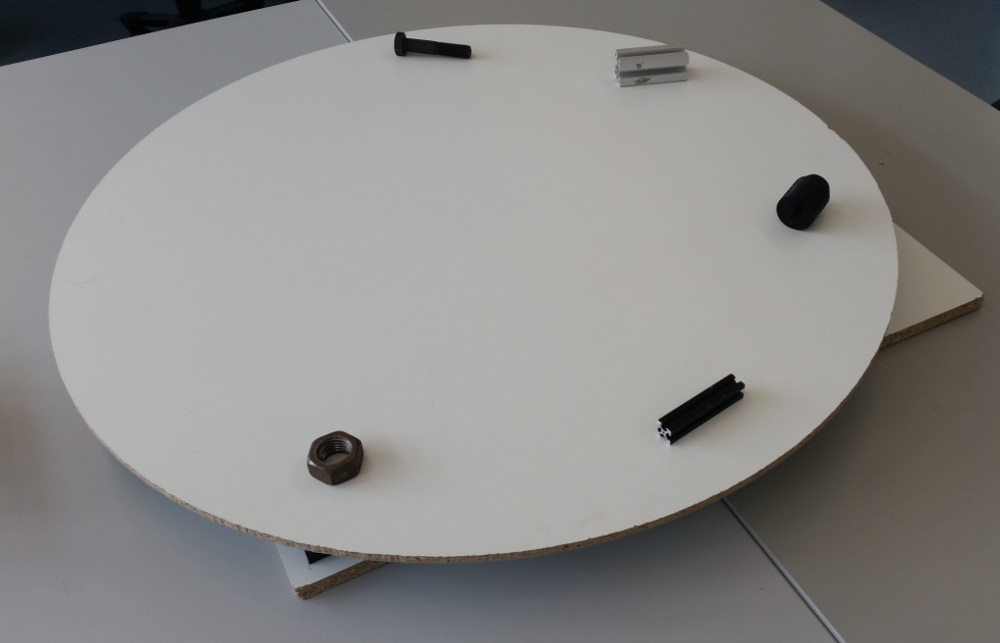
\includegraphics[height = 6cm]{./images/rotating_table.jpg}
	\end{center}
	\caption{Illustration of a rotating table used in the competition.}
	\label{fig:conveyor_belt}
\end{figure}



\paragraph{Manipulation Objects}
The manipulation objects used in this test are defined by the instances described in Table~\ref{tab:Instances}.

\paragraph{Task}
\robin{\st{A single robot is used. The robot is placed by the team in some starting position outside of the arena. Initially the conveyor is switched off (i.e. the belt is not moving) and all objects are put on the belt with a distance between them determined by the TC.}} The task of the robot is to navigate to the location of the rotating table and to grasp all objects from the moving table \robin{\st{belt before they fall off at the other end of the belt. If a turntable is used, the}}. The objects can pass multiple times in front of the robot, until the maximum time for the run is over. The robot is supposed to place the grasped objects on the robot itself. \robin{\st{The task is finished once the robot successfully grasped all objects or the foreseen time of the test has been exceeded.}} 
\par
\robin{\st{There are two options to determine when to switch on the conveyor belt:
The robot starts it itself, using the wireless mechanism or a team member can give a signal to the referees to switch on the conveyor belt.}}
\par
\robin{\st{Teams can decide during the run to give the signal to the referees, e.g. when the robot failed to start it itself. }}


%\subsection{Complexity Options}
%All Complexity Options from BMT apply.


%\subsubsection{Speed Complexity (pick one):}
%
%\begin{itemize}
%\item low speed (bonus factor = +0.0): The conveyor belt speed will be not more than 0.5 cm/s
%\item medium speed (bonus factor = +02):	The conveyor belt speed will be not more than 0.75 cm/s
%\item high speed (bonus factor = +0.4): The conveyor belt speed will be not more than 0.10 cm/s
%\end{itemize}



\paragraph{Rules}
The following rules have to be obeyed:

\begin{itemize}
\item \robin{A single robot is used.}
\item \robin{The robot has to start from outside the arena and to end in the final.}
\item The order in which the teams have to perform will be determined by a draw.
\item The objects are placed on the rotating table before the run starts \robin{by the OC or TC}.
\item \robin{The speed of the rotating table is determined by the OC or TC just before the test starts.}
\item The robot will get the task specification from the referee box.
\item \robin{\st{After the team's robot starts, it must move inside the arena.}}
\item \robin{\st{Either the robot itself starts the conveyor belt, or a team member can give a signal to the referees to switch on the conveyor belt..}}
\item The objects have to be grasped actively from the moving table. \robin{\st{The robot is not allowed e.g. to wait at the end with a particular basket and collect the falling objects from the end of the conveyor belt. Further, wiping the objects to the side is also not allowed.} The robot is not allowed to stop the items with its gripper.}
\item A manipulation object counts as successfully grasped \robin{\st{, if the robot has lifted the object and moved it outside of the area of the conveyor belt}} as specified in Section~\ref{ssec:PlacingObjects}.
\item \robin{A service area counts as successfully reached as defined in Section~\ref{ssec:Navigating}}
\item \robin{\st{The time is stopped when the robot has completed the task.}The run is over when the robot reached the final position or the designated time has expired.}
\item \robin{The score for this test will be calculated as defined in \ref{sec:ScoringAndRanking}.}
\end{itemize}



%
%\subsection{Scoring}
%Points are awarded as follows:
%
%\begin{itemize}
%\item 200 points are awarded for successfully grasping an object from the conveyor belt 
%\item -150 points are given if an object dropped onto the ground, is placed not on the robot itself or dropped from the end of the conveyor..
%\item -100 points are given if the referees had to switch on the belt manually after signalled by a team member, while a working automatic wireless mechanism to switch it on was available.
%\item 50 points are awarded if the task has been fully achieved (when all objects placed on the belt are grasped).
%\end{itemize}
